\chapter{Introduction}
\label{chap:intro}

\section{Motivation}
\label{sect:motivation}
LiDAR senors provide critical depth information for autonomous driving and robotics. The LiDAR intensity maps are often spares and incomplete. Using depht maps as an addtional input is a way to impove the richness and accuracy ot the LiDAR predection. The Pix2Pix network for image-to-image translation offers a promising approch for integrating these modalities. 
\section{Contribution}
This project explores the use of the Pix2Pix network to predict LiDAR intensity maps by leveraging RGB images and depth maps as additional inputs
\section{Related Work}
bpnet depth anything v1 2 and metric change pix2pix to 4 dim input
\chapter{Preparations}
used google colab, pix2pix network getting the right input, pix2pix problems
\begin{figure}[!ht]
	\centering
	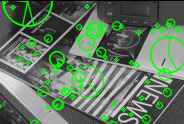
\includegraphics[width=0.9\linewidth]{image.jpg}
	\caption{caption.}
	\label{img:example}
\end{figure}
\chapter{Predicting LIDAR Intensity from RGB and Depth Images}
\section{Setup}
used the bp net it is for depth completion and depth prediction
pix2pix model with modified data loader to get 4 dim. input rgb plus depth
\section{Implementation}
\section{Results}
test run rgb only. depht from depthanything the depth from depthanything v2 and metriv form depthanything v2 6 runs with different solution
\chapter{Conclusion}
\section{Appendix}

\section{References}
bp net work
pix2pix
depth anything v1 2
paper for them 
some for lidar intensity
